%\documentclass[handout]{beamer}
\documentclass{beamer}
\usefonttheme[onlymath]{serif}
\usepackage{xcolor}
\usepackage{graphicx}
\usepackage{siunitx}
\usepackage{amsmath}
\usepackage{MnSymbol}
\usepackage{ulem}
\usepackage{chronosys}
\normalem
\usepackage[procnames]{listings}
\definecolor{keywords}{RGB}{255,0,90}
\definecolor{comments}{RGB}{0,0,113}
\definecolor{red}{RGB}{160,0,0}
\definecolor{green}{RGB}{0,150,0}
\lstset{language=Python, 
        basicstyle=\ttfamily\scriptsize, 
        keywordstyle=\color{keywords},
        commentstyle=\color{comments},
        stringstyle=\color{red},
        showstringspaces=false,
        identifierstyle=\color{green},
        procnamekeys={def,class},
        morekeywords={copy,operate,measure},
        moredelim=[is][\sout]{|}{|},
        moredelim=[is][\uwave]{+}{+}
      }
      
\newcommand{\icol}[1]{% inline column vector
  \left(\begin{smallmatrix}#1\end{smallmatrix}\right)%
}

\newcommand{\irow}[1]{% inline row vector
  \begin{smallmatrix}(#1)\end{smallmatrix}%
}



\usepackage{tikz}
\usetikzlibrary{calc,fpu,fit}
\usetikzlibrary{quantikz}
\usepackage[american]{circuitikz}
\usetikzlibrary{fadings}
\tikzfading[name=fade out, inner color=transparent!0, outer color=transparent!100]
\usetikzlibrary{arrows,decorations.markings}
\usetikzlibrary{arrows,decorations.pathreplacing, patterns, decorations.pathmorphing, positioning}

\newcommand{\AxisRotator}[1][rotate=0]{%
    \tikz \draw[x=.5em,y=1.25em,line width=.2ex,-stealth,#1] (0,0) arc (-150:150:1 and 1);%
  }
  
\usetikzlibrary{shadows}
\tikzset{shaded/.style args={#1:#2:#3 @ #4}{
  left color=#1, right color=#3, middle color=#2, shading angle=#4
}}
\tikzset{pics/.cd, clock/.style args={#1:#2:#3}{code={
%\tikzset{x=1ex, y=1ex, every path/.style={line cap=round}} 
\tikzset{x=0.5ex, y=0.5ex, every path/.style={line cap=round}} 
\shade [shaded=black!75:black!50:black!25 @ 225] circle [radius=13];
\shade [shaded=black!75:black!50:black!25 @ 45]  circle [radius=12.5];
\fill [black!90] circle [radius=12];
\foreach \i [evaluate={\j=90-\i*30; \k=mod(\i,3)==0;\m=int(\i*5);}] in {1,...,12}
  \draw [white, line width=\k ? .2ex : .1ex] (\j:11.5) -- (\j:11-\k) 
    (\j:10) node [anchor=\j, text=black!20, font=\tiny\sffamily]  {\expandafter\uppercase\expandafter{\romannumeral\i}};
\shade [inner color=white, outer color=black, opacity=0.25] circle [radius=12];
\fill [gray!50, rotate=90-#1*30-#2/2-#3/120, 
  rounded corners=.25ex, drop shadow={fill=black, opacity=0.5}]
  (-3/2,3/4) -- (-3/2,-3/4) -- (7,0) -- cycle;
\fill  [gray!50, rotate=90-#2*6-#3/60, 
  rounded corners=0.25ex, drop shadow={fill=black, opacity=0.5}]
  (-3/2,3/4) -- (-3/2,-3/4) -- (11,0) -- cycle;
\fill [red!75!black, drop shadow={fill=black, opacity=0.5}, rotate=90-#3*6] (0,-.05ex) rectangle (11,.05ex);
\shade [shaded=black!50:black!25:black!10 @ 225] circle [radius=1];
\shade [shaded=black!50:black!25:black!10 @ 45] circle [radius=3/4];
\fill [white, opacity=1/16] (0:11) arc (0:180:11) 
.. controls ++(-45:10) and ++(135:10) .. cycle;
}}}

\usepackage{hyperref}

\usepackage{this-macros}

\usetheme{CambridgeUS}
\setbeamertemplate{bibliography item}{\insertbiblabel}
\setbeamertemplate{caption}{\raggedright\insertcaption\par}


\hypersetup{
  bookmarks=true,         % show bookmarks bar?
  unicode=false,          % non-Latin characters in Acrobat’s bookmarks
  pdftoolbar=true,        % show Acrobat’s toolbar?
  pdfmenubar=true,        % show Acrobat’s menu?
  pdffitwindow=false,     % window fit to page when opened
  pdfstartview={Fit},    % fits the width of the page to the window
  pdftitle={A Physicist Peeks into Quantum Architecture},    % title
  pdfauthor={Timothy C. Burt},     % author
  pdfsubject={Quantum information and computer engineering},   % subject of the document
  pdfcreator={Timothy C. Burt},   % creator of the document
  pdfproducer={LaTeX beamer}, % producer of the document
  pdfkeywords={quantum information, quantum physics, computer engineering}, % list of keywords
  pdfnewwindow=true,      % links in new PDF window
  %colorlinks=true,       % false: boxed links; true: colored links
  %linkcolor=blue!60!white,          % color of internal links (change box color with linkbordercolor)
  %citecolor=green,        % color of links to bibliography
  %filecolor=magenta,      % color of file links
  %urlcolor=blue           % color of external links
}

\title{A Physicist Peeks into Quantum Architecture}
\subtitle{Fractured Fairy Tales about Quantum Computer Engineering}
\date{04 October 2019}


\begin{document}
\maketitle

\begin{frame}
\tableofcontents
\end{frame}



\section{Computing}
\subsection{Tall Tales of Truth}
% ----------------------------------------------------------
\begin{frame}
  \frametitle{A Bit of a Story: Evolving a New Computing Technology}
  \begin{itemize}[<+->]
  \item  single-bit memory \visible<6->{(1946)}
    \begin{itemize}[<6->]
    \item \SI{1}{\second} base lifetime of phosphor on cathode ray tube (CRT)
    \end{itemize}
  \item  extend storage lifetime \visible<6->{(1946)}
    \begin{itemize}[<6->]
    \item read charge and rewrite value (regeneration)
    \end{itemize}
  \item improve storage methods \visible<6->{(1947)}
    \begin{itemize}[<6->]
    \item dot-dash and focus-defocus allows 2048 bits stored on 6-inch CRT
    \end{itemize}
  \item enhance manipulation capabilities \visible<6->{(1948)}
    \begin{itemize}[<6->]
    \item \textcolor{orange!80!black}{\emph{design computer around CRT storage device}}
    \item automate bit reset at electronic speeds 
    \item permit random access memory
    \item store 32 32-bit words (1024 bits total), values and instructions
    \end{itemize}
  \item perform computation \visible<6->{(1948)}
    \begin{itemize}[<6->]
    \item only one arithmetic function in hardware, subtraction
    \item application was to find \emph{highest proper divisor} of a number $x$
    \item $x=2^{18}$ took 52 minutes to compute (answer: \num{131072})
    \end{itemize}
  \end{itemize}
  \visible<6->{from history-computer.com~\cite{hist-comp-SSEM}}
\end{frame}
\begin{frame}
  \frametitle{Baby (the SSEM) and its Program}
  \begin{columns}
    \column[T]{0.6\linewidth}
    \begin{figure}
      \centering
      \includegraphics[width=0.73\linewidth]{Graphics/SSEM.jpg}
      \caption{The Small-Scale Experimental Machine (SSEM) computing system nicknamed \emph{Baby} started with a glowing bit on a screen controlled by an electron beam and grew to a vacuum tube-filled system to control \num{1024} bits for a simple calculation}
      \label{fig:Baby}
    \end{figure}

  \column[T]{0.4\linewidth}
    \begin{figure}
      \centering
      \includegraphics[width=0.9\linewidth]{Graphics/first_prog.jpg}
      \caption{\emph{Baby}'s first program --- 7 instructions to find highest proper divisor of a number}
      \label{fig:Baby-1st-program}
    \end{figure}  
  \end{columns}
\end{frame}


% ----------------------------------------------------------
\begin{frame}
  \frametitle{Story of a Killer App}
  \begin{itemize}[<+->]
  \item devise a better way to compute \visible<6->{(1942)}
    \begin{itemize}[<6->]
    \item ``physicist [\ldots] proposed an all-electronic calculating machine''
    \end{itemize}
  \item secure funding \visible<6->{(1943)}
    \begin{itemize}[<6->]
    \item \$7M (2018 dollars) from Army Ordnance Corps R\&D Command
    \end{itemize}
  \item build a complex system \visible<6->{(1945)}
    \begin{itemize}[<6->]
    \item Electronic Numerical Integrator and Computer (ENIAC)
    \item \num{18000} vacuum tubes, $\SI{30}{\meter} \times \SI{2.4}{\meter} \times \SI{0.9}{\meter}$, \SI{27}{ton}, \SI{150}{\kilo\watt} to operate
    \item clock speed of \SI{200}{\micro\second}
    \end{itemize}
  \item incorporate fault tolerance \visible<6->{(1945)}
    \begin{itemize}[<6->]
    \item manual replacement (\SI{15}{min}) of vacuum tubes $\approx$ every \SI{2}{day}
    \item operate below maximum thresholds
    \end{itemize}
  \item execute application \visible<6->{(1945--1955)}
    \begin{itemize}[<6->]
    \item artillery ballistic tables
    \item single-trajectory calculation time reduction from \SI{20}{hr} to \SI{30}{\second}
    \end{itemize}
  \end{itemize}
  \visible<6->{from various sources~\cite{chm-ENIAC, Crystal-Fire}}
\end{frame}


\subsection{Stacking Layers}
% ----------------------------------------------------------
\begin{frame}
  \frametitle{A Classical Computing Stack}

  \begin{columns}
    \column[T]{0.65\linewidth}
    \includegraphics[width=0.95\linewidth]{%
      Graphics/Abstract-Classical-Computing-Stack.jpg}
    
    Image from StackExchange \url{https://electronics.stackexchange.com/q/353915}

  
    \column[T]{0.35\linewidth}
    \begin{block}{Outside-in}
      \begin{enumerate}
      \item Applications
      \item Physical foundations
      \item Building between the extremes
      \end{enumerate}
    \end{block}
  \end{columns}
\end{frame}


% ----------------------------------------------------------
\begin{frame}
  \frametitle{Bits are Mother Nature's Children}
  Devices, like the transistor, behave based on physical principles.
  Engineers and scientists use their understanding of Mother Nature to
  craft useful things.
  
  \begin{columns}
    % col 1
    \column[T]{0.5\linewidth}
    \includegraphics[width=0.75\linewidth]{Graphics/CHM-Transistor-picture.jpg}
    % col 1
    \column[T]{0.5\linewidth}
    \includegraphics[width=0.95\linewidth]{Graphics/CHM-Transistor-diagram-physics.jpg}
    images from Computer History Museum~\cite{CHM-Transistor-article}
  \end{columns}

\end{frame}


% ----------------------------------------------------------
\begin{frame}
  \frametitle{Gates and Universal Computing}
  Gates are one way to represent actions within a circuit, modifying inputs to output. Some logic gate sets are known to be Turing complete ---  capable of universal computing~\cite{Sheffer, electronic-tutorials}. 
  \begin{itemize}
  \item NAND \tikz \draw (0,0) node[scale=0.5, american nand port] (nand)
    {} (nand.in 1) node [anchor=east] {$a$} (nand.in 2) node [anchor=east]
    {$b$} (nand.out) node [anchor=west] {$\lnot (a \land b)$};
  \item NOR \tikz \draw (0,0) node[scale=0.5, american nor port] (nor)
    {} (nor.in 1) node [anchor=east] {$a$} (nor.in 2) node [anchor=east]
    {$b$} (nor.out) node [anchor=west] {$\lnot (a \lor b)$};
  %\item NOR \tikz \node[scale=0.5] [american nor port] {};
    
  \item AND with NOT \tikz{ \draw (0,0) node[scale=0.5, american and port]
      (and) {} (and.in 1) node [anchor=east] {$a$} (and.in 2) node
      [anchor=east] {$b$} (and.out) node [anchor=west] {$a \land b$} ; \draw
      (2.5,0) node [scale=0.5, american not port] (not) {} (not.in) node
      [anchor=east] {$a$} (not.out) node [anchor=west] {$\lnot a$};} 
  \item OR with NOT \tikz{ \draw (0,0) node[scale=0.5, american or port]
      (or) {} (or.in 1) node [anchor=east] {$a$}  (or.in 2) node
        [anchor=east] {$b$}  (or.out) node [anchor=west] {$a \lor b$}; \node at (2.0,0) [scale=0.5] [american not port] {};} 
  \item AND with OR with NOT \tikz{ \node[scale=0.5] [american and port] {}; \node at (1,0) [scale=0.5] [american or port] {}; \node at (1.75,0) [scale=0.5] [american not port] {};} 
  %\item Controlled-controlled NOT (Toffoli)
  %\item $A \land \lnot B$
  %\item $B \land \lnot A$
  %\item $A \lor \lnot B$
  %\item $B \lor \lnot A$
  \end{itemize}
\end{frame}



% ----------------------------------------------------------
\begin{frame}
  \frametitle{Simple Arithmetic Circuit: Add with Carry}
  Too much to add two bits? No --- marvelous electronic devices are borne
  from such humble beginnings
  
  \begin{circuitikz}
    \draw %
    % gate layout
    (1,0) node[xor port] (xor1) {} %
    (3,-0.5) node[xor port] (xor2) {} %
    (3,-2) node[and port] (and1) {} %
    (3,-3.5) node[and port] (and2) {} %
    (5,-2.75) node[or port] (or1) {} %
    % connections
    (xor1.in 1) to [short, -o] ++(-1,0) %
    ($(xor1.in 1)+(-1,0)$)  node [anchor=east] {$a$} %
    (xor1.in 2) to [short, -o] ++(-1,0) %
    ($(xor1.in 2)+(-1,0)$)  node [anchor=east] {$b$} %
    (xor2.in 2) to [short, -o] ++(-3,0) %
    ($(xor2.in 2)+(-3,0)$)  node [anchor=east] {$C_{\text{in}}$} %
    (xor1.out) -| (xor2.in 1) %
    (and2.in 1) -| (xor1.in 1) node [circ] {} %
    (and2.in 2) -| ($(xor1.in 2)+(-0.5,0)$) node [circ] {} %
    (and1.in 1) -| (xor1.out) node [circ] {} %
    (and1.in 2) -| ($(xor2.in 2)+(-1,0)$) node [circ] {} %
    (and1.out) -| (or1.in 1) %
    (and2.out) -| (or1.in 2) %
    (or1.out) to[short, -o] ++(0.25,0) node [right] {$C_{\text{out}}$}
    (xor2.out) to[short, -o] ++(2.25,0) node [right] {$S$}
    ;
    %(xorAB.in 1) node [anchor=east] {$a$} %
    %(xorAB.in 2) node [anchor=east] {$b$} %
    %(xorAB.out) to node [and port] {};
  \end{circuitikz}
\end{frame}


% ----------------------------------------------------------
\begin{frame}[fragile]
  \frametitle{Speaking its Language for Computational Conversations}
  High-level, expressive language is translated to more primitive
  operations and to \emph{supported} instructions for a given system to
  carry out and return results.
  
  \begin{lstlisting}
    def simpleFunction(inValOne, inValTwo):
        # set x and y to the inputs
        x = copy(inValOne) 
        y = copy(inValTwo)
        # perform operation on the inputs (e.g. add)
        operate(x, y, out=z)
        # obtain the output of the operation
        s = measure(z)
        return s

    # Example script
    out = simpleFunction(2,2)
    print('result = {}'.format(out)) # Result = a reproducible value
  \end{lstlisting}
  
\end{frame}


\section{Quantum Computing}


% ----------------------------------------------------------
%-req-%\usetikzlibrary{shadows}

%-req-%\newcommand{\AxisRotator}[1][rotate=0]{%
%-req-%    \tikz \draw[x=.5em,y=1.25em,line width=.2ex,-stealth,#1] (0,0) arc (-150:150:1 and 1);%
%-req-%  }

%-req-%\tikzset{shaded/.style args={#1:#2:#3 @ #4}{
%-req-%  left color=#1, right color=#3, middle color=#2, shading angle=#4
%-req-%}}
%-req-%\tikzset{pics/.cd, clock/.style args={#1:#2:#3}{code={
%-req-%%\tikzset{x=1ex, y=1ex, every path/.style={line cap=round}} 
%-req-%\tikzset{x=0.5ex, y=0.5ex, every path/.style={line cap=round}} 
%-req-%\shade [shaded=black!75:black!50:black!25 @ 225] circle [radius=13];
%-req-%\shade [shaded=black!75:black!50:black!25 @ 45]  circle [radius=12.5];
%-req-%\fill [black!90] circle [radius=12];
%-req-%\foreach \i [evaluate={\j=90-\i*30; \k=mod(\i,3)==0;\m=int(\i*5);}] in {1,...,12}
%-req-%  \draw [white, line width=\k ? .2ex : .1ex] (\j:11.5) -- (\j:11-\k) 
%-req-%    (\j:10) node [anchor=\j, text=black!20, font=\tiny\sffamily]  {\expandafter\uppercase\expandafter{\romannumeral\i}};
%-req-%\shade [inner color=white, outer color=black, opacity=0.25] circle [radius=12];
%-req-%\fill [gray!50, rotate=90-#1*30-#2/2-#3/120, 
%-req-%  rounded corners=.25ex, drop shadow={fill=black, opacity=0.5}]
%-req-%  (-3/2,3/4) -- (-3/2,-3/4) -- (7,0) -- cycle;
%-req-%\fill  [gray!50, rotate=90-#2*6-#3/60, 
%-req-%  rounded corners=0.25ex, drop shadow={fill=black, opacity=0.5}]
%-req-%  (-3/2,3/4) -- (-3/2,-3/4) -- (11,0) -- cycle;
%-req-%\fill [red!75!black, drop shadow={fill=black, opacity=0.5}, rotate=90-#3*6] (0,-.05ex) rectangle (11,.05ex);
%-req-%\shade [shaded=black!50:black!25:black!10 @ 225] circle [radius=1];
%-req-%\shade [shaded=black!50:black!25:black!10 @ 45] circle [radius=3/4];
%-req-%\fill [white, opacity=1/16] (0:11) arc (0:180:11) 
%-req-%.. controls ++(-45:10) and ++(135:10) .. cycle;
%-req-%}}}
  
\begin{frame}
  \frametitle{Planck's Call to Action}

  The difference between classical physics and quantum
  physics is Planck's constant $\hbar$ (technically, $i\hbar$). %
  \mbox{}
  \vfill

  \begin{tikzpicture}
    \node (hbarapprox) at (-2.0,1.0) {\Huge $\hbar \approx$};    
    \input{Graphics/coffee-cup-tikz}
    \draw[->, >=stealth, gray] (0,-0.2) -- ++(0,2);
    \draw[ultra thick] (0,1.5) node {\AxisRotator[rotate=-90]};
    \node [right] (rot) at (0.5, 1.5) {rotating a cup a billionth of a turn
      \ldots};
    \node[right] (clock) at (2.0,1.0) {\ldots over the lifetime of the
      universe!};
    
    \pic at (5.5,-0.5) {clock={6:36:34}};
    \node[below] (hbar) at ((5.5,-1.5) {$\hbar \equiv \SI{6.62607015 e-34}{\joule\second}$};
  \end{tikzpicture}
\end{frame}


% ----------------------------------------------------------
\begin{frame}
  \frametitle{Finding the Electron in Electronics}

  Transistor sizes from centimeters to nanometers
  
  \includegraphics[width=0.2\linewidth]{Graphics/CHM-Transistor-picture.jpg}
  \includegraphics[width=0.35\linewidth]{Graphics/SE-Bell-junction.png}
  \includegraphics[width=0.20\linewidth]{Graphics/SE-bipolar-transistor.png}
  \includegraphics[width=0.20\linewidth]{Graphics/SE-3nm-channel-transistor.jpg}

  \begin{columns}
    % SET
    \column[T]{0.25\linewidth}
    Single electron transport (NIST)
  
    \includegraphics[width=0.95\linewidth]{Graphics/SE-NIST-set1.png}

    % electron angular momentum
    \column[T]{0.75\linewidth}
    \begin{block}{Hello Planck}
      orbit angular momentum of electron in lowest energy state of hydrogen
      is $\sqrt{2} \hbar$
    \end{block}
  \end{columns}

  images from various sources~\cite{CHM-Transistor-article, Lost-history-transistor, NRL-nanoelectronics,
    PhysOrg-3nm-channel-transistor, NIST-Single-electron-transport}
\end{frame}


% ----------------------------------------------------------
\begin{frame}
  \frametitle{Peering Into the Future of Quantum Information}
  \mbox{}%
  \vfill
  \begin{quote}
    History does not repeat itself, but it often rhymes. \\%
    \mbox{}\hfill --- Anonymous (often misattributed to Mark Twain~\cite{QI-History-Rhymes})
  \end{quote}
  \vfill %
  \mbox{}
\end{frame}



\subsection{Surveying the Strata}
% ----------------------------------------------------------
\begin{frame}
  \frametitle{A Qubit of a Story}
  
  \begin{itemize}[<+->]
  \item generalize Shannon information theory for quantum systems \visible<6->{(1976)}
    \begin{itemize}[<6->]
    \item $n$ quantum bits (qubits) \emph{access} more information that $n$
      bits
    \item at most $n$ classical bits can be \emph{output} from $n$ qubits
    \end{itemize}
  \item envision computation with quantum resources \visible<6->{(1980--1985)}
    \begin{itemize}[<6->]
    \item universal quantum computer justified (Deutsch) 
    \end{itemize}
  \item develop algorithms with quantum-advantage over classical \visible<6->{(1990s)}
    \begin{itemize}[<6->]
    \item prime factorization (Shor's algorithm) 
    \item database search (Grover's algorithm)
    \end{itemize}
  \item demonstrate quantum component \visible<6->{(1995)}
    \begin{itemize}[<6->]
    \item controlled not gate with trapped ions 
    \end{itemize}
  \item perform computation \visible<6->{(2016)}
    \begin{itemize}[<6->]
    \item \textcolor{orange!80!black}{\emph{probabilistic} factorization of \num{15} \emph{without foreknowledge} of factors}
    \end{itemize}
  \end{itemize}
  \visible<6->{various sources~\cite{NIST-QComp, Wikipedia-Timeline-QComp}}
\end{frame}


% ----------------------------------------------------------
\begin{frame}
  \frametitle{Sisyphus at the Gate of Five Ions}
  \begin{columns}
    % CNOT gate
    \column[T]{0.5\linewidth}
    Laboratory-sized quantum gate using bulk optics 
    \begin{figure}
      \centering
      \includegraphics[width=0.95\linewidth]{Graphics/nist_ionstorage1996.jpg}      
      \caption{Demonstrating a controlled not gate using trapped
        ions (NIST)~\cite{NIST-Q-Logic-Gates}}
    \end{figure}
    
    % Shor algorithm for 15
    \column[T]{0.5\linewidth}
    \begin{figure}
      \centering
    \includegraphics[width=0.95\linewidth]{Graphics/PW-2016-03-04-ion-trap-3-Shor15.jpg}
      
      \caption{Five ion qubits used Shor's algorithm to factor the number
        15~\cite{PW-Shor-factor-15}}
    \end{figure}
  \end{columns}

\end{frame}


% ----------------------------------------------------------
\begin{frame}
  \frametitle{Quantum Computing Stacks}

  \begin{columns}
    % SC stack
    \column[T]{0.45\linewidth}
    \begin{figure}
      \centering
      \includegraphics[width=0.95\linewidth]{Graphics/QComp-Stack-Nature.jpg}
      \caption{A notional stack for quantum computers from
        IBM~\cite{SC-QComp-stack}}   
    \end{figure}
    
    % ACM stack
    \column[T]{0.55\linewidth}
    \begin{figure}
      \centering
      \includegraphics[width=0.95\linewidth]{Graphics/ACM-QComp-stack.png}
      \caption{A more detailed view of quantum computer architecture from
        the Association for Computing Machinery~\cite{acm-qcomp-blueprint}}
    \end{figure}
    
  \end{columns}
  
\end{frame}



\subsection{Physical Basis}
% ----------------------------------------------------------

%-req-%\newcommand{\icol}[1]{% inline column vector
%-req-%  \left(\begin{smallmatrix}#1\end{smallmatrix}\right)%
%-req-%}
%-req-%\newcommand{\irow}[1]{% inline row vector
%-req-%  \begin{smallmatrix}(#1)\end{smallmatrix}%
%-req-%}

\begin{frame}
  \frametitle{A Superposition of What?}
  \begin{columns}
    % Abstract
    \column{0.5\linewidth} In the abstract, a qu\textbf{\uline{b}}it is a complex, linear
    superposition of two (exclusive and complete) states of a system in a
    two-dimensional Hilbert space --- \emph{\textbf{not} a vector in three
      dimensions} 
    \begin{equation*}
      \ket{\psi} = \alpha\ket{0} + \beta\ket{1} = \alpha\icol{1\\0} +
      \beta\icol{0\\1} 
    \end{equation*}

    
    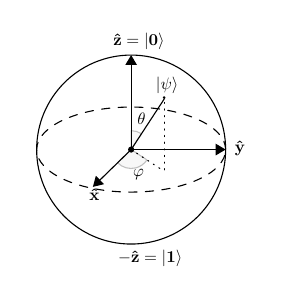
\begin{tikzpicture}[scale=0.6, transform shape,
      line cap=round, line join=round, >=Triangle]
      \clip(-2.19,-2.49) rectangle (2.66,2.58);
      \draw [shift={(0,0)}, lightgray, fill, fill opacity=0.1] (0,0) -- (56.7:0.4) arc (56.7:90.:0.4) -- cycle;
      \draw [shift={(0,0)}, lightgray, fill, fill opacity=0.1] (0,0) -- (-135.7:0.4) arc (-135.7:-33.2:0.4) -- cycle;
      \draw(0,0) circle (2cm);
      \draw [rotate around={0.:(0.,0.)},dash pattern=on 3pt off 3pt] (0,0) ellipse (2cm and 0.9cm);
      \draw (0,0)-- (0.70,1.07);
      \draw [->] (0,0) -- (0,2);
      \draw [->] (0,0) -- (-0.81,-0.79);
      \draw [->] (0,0) -- (2,0);
      \draw [dotted] (0.7,1)-- (0.7,-0.46);
      \draw [dotted] (0,0)-- (0.7,-0.46);
      \draw (-0.08,-0.3) node[anchor=north west] {$\varphi$};
      \draw (0.01,0.9) node[anchor=north west] {$\theta$};
      \draw (-1.01,-0.72) node[anchor=north west] {$\mathbf {\hat{x}}$};
      \draw (2.07,0.3) node[anchor=north west] {$\mathbf {\hat{y}}$};
      \draw (-0.5,2.6) node[anchor=north west] {$\mathbf {\hat{z}=|0\rangle}$};
      \draw (-0.4,-2) node[anchor=north west] {$-\mathbf {\hat{z}=|1\rangle}$};
      \draw (0.4,1.65) node[anchor=north west] {$|\psi\rangle$};
      \scriptsize
      \draw [fill] (0,0) circle (1.5pt);
      \draw [fill] (0.7,1.1) circle (0.5pt);
    \end{tikzpicture}
    
    % Physical
    \column{0.5\linewidth}
    \begin{block}{Atomic (spin)}
      \vspace*{-\baselineskip}
      \begin{align*}
        \ket{\psi}_{\text{electron-spin}} &= \alpha\ket{\uparrow}_{\text{el}} +
                                       \beta\ket{\downarrow}_{\text{el}} %
        \\ %
        \ket{\psi}_{\text{nuclear-spin}} &= \alpha\ket{\uparrow}_{\text{nuc}} +
                                      \beta\ket{\downarrow}_{\text{nuc}} %
      \end{align*}
    \end{block}
    
    \begin{block}{Photonic (polarization and number)}
      \vspace*{-\baselineskip}
      \begin{align*}
        \ket{\psi}_{\text{photon-pol}} &= \alpha\ket{\nwsearrow}_{\text{ph}} +
                                       \beta\ket{\neswarrow}_{\text{ph}} %
        \\ %
        \ket{\psi}_{\text{photon-num}} &= \alpha\ket{0}_{\text{ph}} +
                                      \beta\ket{1}_{\text{ph}} %
      \end{align*}
    \end{block}
    
    \begin{block}{Electronic (charge, current)}
      \vspace*{-\baselineskip}
      \begin{align*}
        \ket{\psi}_{\text{chg}} &= \alpha\ket{0}_{\text{chg}} +
                                  \beta\ket{2e}_{\text{chg}} %
        \\ %
        \ket{\psi}_{\text{curr}} &= \alpha\ket{\circlearrowright}_{\text{curr}} +
                                   \beta\ket{\circlearrowleft}_{\text{curr}} %
      \end{align*}
    \end{block}
  \end{columns}
\end{frame}


% ----------------------------------------------------------
\begin{frame}
  \frametitle{The Delicate, Competitive Dance of Quantum Information}
  \begin{itemize}
  \item Isolation
    \begin{itemize}
    \item Generated quantum states are fragile
    \item Noise destroys, or at least complicates, their coherent nature
    \item Segregation from environment and other systems is paramount \ldots
    \end{itemize}

  \item Interaction
    \begin{itemize}
    \item \ldots except splendid isolation leaves no means for control
    \item Manipulation and detection of quantum states is necessary for
      utility
    \item Quantum systems need to influence one another and another
      and \ldots
    \end{itemize}

  \item Interconnection
    \begin{itemize}
    \item \ldots a completely other
    \item Collections of heterogeneous quantum systems must inter-communicate
      quantum information  
    \end{itemize}

  \end{itemize}
\end{frame}


% ----------------------------------------------------------
\begin{frame}
  \frametitle{Pardigms Lost}
  \begin{itemize}
  \item Measurement is not deterministic
    \begin{itemize}
    \item Probabilistic results
    \item \emph{Logic structure of quantum physics is different}
      \begin{itemize}
      \item $X \land P \land X \neq X \land X \land P$
      \end{itemize}
    \end{itemize}
  \item Short lifetimes of stability
    \begin{itemize}
    \item transistor: $\sim \SI{e9}{yr} \approx \SI{e16}{\second}$
    \item qubit: $\sim \SI{e-3}{\second}$
    \item \emph{Ultra-fast operation of quantum devices is necessary}
    \end{itemize}
  \item No-cloning theorem
    \begin{itemize}
    \item \emph{An arbitrary quantum state cannot be copied}
    \end{itemize}
  \end{itemize}
  \begin{block}{Paradigms Gained}
    Teleportation, increased correlations, computational speedup, etc.
  \end{block}
\end{frame}


% ----------------------------------------------------------
\begin{frame}
  \frametitle{Quantum Gates and Universal Quantum Computing}
  $H, S, T,$ and CNOT are a universal set of quantum gates
  \begin{columns}
    % Col 1
    \column[T]{0.45\linewidth}
    %\begin{itemize}
    %\item ``quantum circuits subsume classical circuits''~\cite[\S 4.5]{QCQI-Nielsen}
    %\item 
    %\end{itemize}

    % Phase (S)
    \begin{block}{Phase}
      \begin{quantikz}
        \lstick{\ket{1}} & \gate{S} & \rstick{$e^{i\pi/2}\ket{1}$} \qw
      \end{quantikz}
        \begin{equation*}
          \begin{pmatrix}
            1 & 0 \\
            0 & i
          \end{pmatrix}
        \end{equation*}
    \end{block}

    % $\pi/8$
    \begin{block}{$T$ (also known as $\pi/8$)}
      \begin{quantikz}
        \lstick{\ket{1}} & \gate{T} & \rstick{$e^{i\pi/4}\ket{1}$} \qw
      \end{quantikz}  
        \begin{equation*}
          \begin{pmatrix}
            1 & 0 \\
            0 & e^{i\pi/4}
          \end{pmatrix}
          = %
          e^{i\pi/8}
          \begin{pmatrix}
            e^{-i\pi/8} & 0 \\
            0 & e^{i\pi/8}
          \end{pmatrix}
        \end{equation*}
    \end{block}

    % Col 2
    \column[T]{0.45\linewidth}
    % Hadamard (H)
    \begin{block}{Hadamard}
      \begin{quantikz}
        \lstick{\ket{0}} & \gate{H} & \rstick{$(\ket{0} + \ket{1})/\sqrt{2}$} \qw
      \end{quantikz}   
        \begin{equation*}
          \begin{pmatrix}
            1 & 1 \\
            1 & -1
          \end{pmatrix}
        \end{equation*}
    \end{block}

    % Controlled not 
    \begin{block}{CNOT (two-qubit gate)}
      \begin{tiny}
        \begin{quantikz}
          \lstick{$\ket{c}$} & \ctrl{1} & \rstick{$\ket{c}$} \qw \\ %
          \lstick{$\ket{t}$} & \targ{} & \rstick{$\ket{c}\ket{t\oplus c}$}\qw
        \end{quantikz}
      \end{tiny}
      \begin{Tiny}
        \begin{equation*}
          \begin{pmatrix}
            1 & 0 & 0 & 0 \\
            0 & 1 & 0 & 0 \\
            0 & 0 & 0 & 1 \\
            0 & 0 & 1 & 0 \\
          \end{pmatrix}
        \end{equation*}
      \end{Tiny}
      \vspace*{-\baselineskip}
    \end{block}

  \end{columns}
\end{frame}


% ----------------------------------------------------------
\begin{frame}
  \frametitle{Get Sum Mod Quantum}
  Build-up of quantum circuit to compute $(a+b) \mod N$
  \begin{columns}
    % sum and carry
    \column[T]{0.35\linewidth}
    \includegraphics[width=0.95\linewidth]{Graphics/Q-Arithmetic-SUM-and-CARRY.png}

    % adder
    \column[T]{0.65\linewidth}
    \includegraphics[width=0.95\linewidth]{Graphics/Q-Arithmetic-ADDER.png}
  \end{columns}
  
  \includegraphics[width=0.75\linewidth]{Graphics/Q-Arithmetic-ADDERMOD.png}

  image credit~\cite{arXiv:9511018}
\end{frame}


% ----------------------------------------------------------
\begin{frame}
  \frametitle{Circuit Optimation for Application}
  Optimization takes advantage of allowed transformations (e.g. commutation
  and cancellation) to reduce gate count, decrease circuit depth,
  accommodate gate set, etc. 
  \begin{columns}
    \column[T]{0.65\linewidth}
    \includegraphics[width=\linewidth]{Graphics/Q-cancellation-optimizer.png}

    \column[T]{0.35\linewidth}  
    \includegraphics[width=\linewidth]{Graphics/Q-cancellation-optimized.png}
  \end{columns}
  \begin{center}
    \vspace*{-\baselineskip}
    \includegraphics[width=0.55\linewidth]{Graphics/Rotation-gate-reduction-VOQC.png}
  \end{center}

  Verified Optimizer for Quantum Computing (VOQC)~\cite{VOQC}
\end{frame}



\subsection{Quantum Computer Engineering}
% ----------------------------------------------------------
% ----------------------------------------------------------
\begin{frame}[fragile]
  \frametitle{A Foreign Language to Quantum Mother Nature}
  Basic quantum mechanics does not allow common, classical behavior such as
  copying and deterministic measurement.
  \begin{itemize}
  \item No-cloning theorem: Cannot copy an unknown state!
  \item Measurment postulate: Random selection of eigenstates!
  \end{itemize}
  
  \begin{lstlisting}
    def simpleFunction(inValOne, inValTwo):
        # set x and y to the inputs
        # ==========> NO-CLONING THEOREM
        x = |copy|(inValOne) 
        y = |copy|(inValTwo)
        # perform operation on the inputs (e.g. add)
        operate(x, y, out=z)
        # obtain the output of the operation
        # ==========> MEASUREMENT POSTULATE
        s = +measure+(z)
        return s

    # Example script
    out = simpleFunction(2,2)
    print('result = {}'.format(out)) # Result = ??? 
  \end{lstlisting}
\end{frame}

% ----------------------------------------------------------
\begin{frame}
  \frametitle{Applications of Quantum Information}
  \begin{scriptsize}
      \begin{columns}
    % col 1
    \column[T]{0.45\linewidth}
    % sensing
    \begin{block}{Sensing}
      \begin{itemize}
      \item spatial measurements (e.g. translation, rotation)
      \item metrology of physical quantities (e.g. electric field, gravity)
      \item imaging (e.g. ghost imaging, computational imaging)
      \end{itemize}
    \end{block}
    
    % computing
    \begin{block}{Computing}
      \begin{itemize}
      \item factor prime numbers (e.g. crack encryption)
      \item database search
      \item optimization (e.g. traveling salesman problem)
      \item machine learning
      \end{itemize}
    \end{block}
    % col 2
    \column[T]{0.45\linewidth}

    % communication
    \begin{block}{Communication}
      \begin{itemize}
      \item provably-secure key generation and distribution
        (e.g. cryptography) 
      \item network security using untrusted nodes
      \item transaction protection (e.g. financial, voting)
      \item collective exposure (e.g. secret sharing)
      \item non-repudiation (e.g. contracts)
      \end{itemize}
    \end{block}

    % simulation
    \begin{block}{Simulation}
      \begin{itemize}
      \item chemical reactions
      \item genetics
      \item pharmaceuticals
      \end{itemize}
    \end{block}

    
  \end{columns}
  \end{scriptsize}
\end{frame}


% ----------------------------------------------------------
\begin{frame}
  \frametitle{Quantum Hardware}
  Quantum-specific aspects constitute a small portion of a system
  \begin{columns}
    % Column 1
    \column[T]{0.33\linewidth}
    \begin{figure}
      \centering
    \includegraphics[width=0.75\linewidth]{Graphics/CEO-Forum_IBM-50Q-system_thumb.jpg}
      \caption{IBM Q dilution refrigerator (\SI{15}{\milli\kelvin}) and interface wiring to 50 superconducting charge qubits (transmons)~\cite{IBMQ-blog}}
    \end{figure}

    % Column 2
    \column[T]{0.33\linewidth}
    \begin{figure}
      \centering
      \caption{Xanadu cluster state photonic computer on chip (electronics
        and controls not shown)~\cite{Xanadu-Hardware}}
      \includegraphics[width=0.48\linewidth]{Graphics/xanadu-chips-circle.png}    
      \includegraphics[width=0.48\linewidth]{Graphics/xanadu-control-systems.jpg}
    \end{figure}    % Column 3
    \column[T]{0.33\linewidth}
    \begin{figure}
      \centering
      \includegraphics[width=0.95\linewidth]{Graphics/surface_trap-monroe-gallery.jpg}
      \caption{IonQ and Joint Quantum Institute atomic ion trap (laser
        cooling, atomic manipulation controls, and electronics not
        shown)~\cite{JQI-15M-NSF-news}}
    \end{figure}
  \end{columns}
\end{frame}

% ----------------------------------------------------------
\begin{frame}
  \frametitle{Problem-Specific Qubit Scaling}
  Problem: Factor 2048-bit number

  Solution: Design device for Shor's algorithm with logical qubits, ancilla
  generation, connections, surface code error correction, and imperfect
  device yield~\cite{acm-qcomp-blueprint}
    
  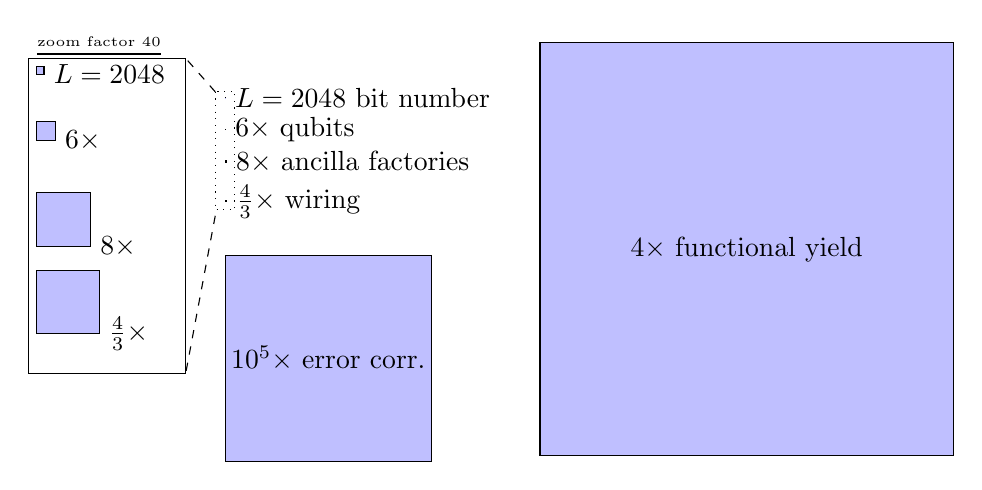
\begin{tikzpicture}[x=1mm, y=1mm, qubits/.style={fill = blue!25}]
    \def\baseLen{0.025}
    \def\shiftLen{1}
    \draw [qubits] (0,0) rectangle %
    +(\baseLen, -\baseLen) %
    node [right] {$L=2048$ bit number}; %
    
    \draw [qubits] (0,-4*\shiftLen) rectangle %
    +(sqrt 6*\baseLen, -sqrt 6*\baseLen) %
    node [right] {$6\times$ qubits}; %
    
    \draw [qubits] (0,-8*\shiftLen) rectangle %
    +(sqrt 48*\baseLen, -sqrt 48*\baseLen) %
    node [right] {$8\times$ ancilla factories}; %
    
    \draw [qubits] (0,-13*\shiftLen) rectangle %
    +(sqrt 64*\baseLen, -sqrt 64*\baseLen) %
    node [right] {$\frac{4}{3}\times$ wiring}; %
    
    \draw [qubits] (0,-20*\shiftLen) rectangle %
    +(1049*\baseLen, -1049*\baseLen) %
    node [midway] {$\num{e5}\times$ error corr.};
    
    \draw [qubits] (40*\shiftLen,7*\shiftLen) rectangle %
    +(2100*\baseLen, -2100*\baseLen) %
    node [midway] {$4\times$ functional yield}; %

    \coordinate (ULsmall) at (-50*\baseLen, 30*\baseLen);
    \coordinate (LLsmall) at (-50*\baseLen, -15*\shiftLen);
    \draw [dotted] (ULsmall) rectangle +(100*\baseLen, -15*\shiftLen);

    % Increase base length 
    \def\baseLen{1}
    % Make the zoom box
    \draw (-25*\baseLen, 5*\baseLen) rectangle +(20*\baseLen,
    -40*\shiftLen);
    \draw [dashed] (ULsmall) -- (-5*\baseLen, 5*\baseLen);
    \draw [dashed] (LLsmall) -- (-5*\baseLen, -35*\baseLen);
    \node [label=above:\emph{\tiny{zoom factor 40}}] (zoomBox) at (-16*\baseLen, 3*\shiftLen) {};
    \draw [qubits] (-24*\baseLen, 4*\shiftLen) rectangle %
    +(\baseLen, -\baseLen) %
    node [right] {$L=2048$}; %
    
    \draw [qubits] (-24*\baseLen,-3*\shiftLen) rectangle %
    +(sqrt 6*\baseLen, -sqrt 6*\baseLen) %
    node [right] {$6\times$}; %
    
    \draw [qubits] (-24*\baseLen,-12*\shiftLen) rectangle %
    +(sqrt 48*\baseLen, -sqrt 48*\baseLen) %
    node [right] {$8\times$}; %
    
    \draw [qubits] (-24*\baseLen,-22*\shiftLen) rectangle %
    +(sqrt 64*\baseLen, -sqrt 64*\baseLen) %
    node [right] {$\frac{4}{3}\times$}; %
  \end{tikzpicture}
\end{frame}


% ----------------------------------------------------------
\begin{frame}
  \frametitle{Ready to be QIST}
  {\footnotesize %
    Contributors to Quantum Information Science and Technology (QIST) will
    come together from a range of backgrounds, few of which will be quantum
    physics. %
  }

  \mbox{}\hfill%
  \includegraphics[width=0.85\linewidth]{Graphics/QInfo-tree-crop.pdf} %
  \hfill\mbox{}
\end{frame}



% ----------------------------------------------------------
\begin{frame}
  \frametitle{Omne rerum principia parva sunt\footnote{All beginnings are small}}
  \mbox{}\vfill%
  \begin{quote}
    Quantum theory provides us with a striking illustration of the fact
    that we can fully understand a connection though we can only speak of
    it in images and parables.\\
    --- Werner Heisenberg in Physics and Beyond: Encounters and Conversation
  \end{quote}
  \vfill\mbox{}
\end{frame}


\section{References}


\begin{frame}
  \frametitle{Further Reading}
  \begin{itemize}
  \item Quantum Computing Reports, Tools~\cite{qcomprpt-tools}
  \item Quantum Programming (Wikipedia)~\cite{wikipedia-qcomp}
  \item Quantum Computing: An Overview Across the System Stack~\cite{arxiv:1905.07240}
  \item Full-Stack, Real-System Quantum Computer Studies~\cite{arxiv:1905:11349} 
    \begin{itemize}
    \item ``the purpose of our work is to build insights in how architecture and compiler design choices can best support the different technologies''
    \end{itemize}
  \item Quantum Networks for Elementary Arithmetic Operations~\cite{arXiv:9511018}
  \item Automated optimization of large quantum circuits with continuous parameters~\cite{npj-s41534-018-0072-4}
  \end{itemize}
\end{frame}


\begin{frame}
  \frametitle{Abstract}
  In analogy with a classical computing stack, aspects of quantum information processing are explored from physical underpinnings of devices to application programming. Particular emphasis is given to the subsystems between these extremes regarding challenges to realize them such as scaling and error correction. Potential applications that could benefit from quantum processing and the skills of computer engineering are discussed, especially those that might be considerably more near-term than a universal quantum computer. As Tank said in `Matrix'~\cite{movie-Matrix}, ``It’s a very exciting time. We got a lot to do. We gotta get to it.''
\end{frame}


\begin{frame}[allowframebreaks]{Bibliography}
  \begin{thebibliography}{99}
  \bibitem{hist-comp-SSEM} %
    \emph{SSEM (Small Scale Experimental Machine)}, %
    \url{https://history-computer.com/ModernComputer/Electronic/SSEM.html}

  \bibitem{acm-qcomp-blueprint} %
    \emph{A Blueprint For Building a Quantum Computer}, %
    Rodney Van Meter and Clare Horsman, %
    Communications of the ACM, Vol. 56 No. 10, Pages 84-93, (2013) %
    \url{https://m-cacm.acm.org/magazines/2013/10/168172-a-blueprint-for-building-a-quantum-computer/fulltext}

  \bibitem{chm-ENIAC} %
    \emph{ENIAC (Birth of the Computer)}, %
    Computer History Museum, %
    \url{https://www.computerhistory.org/revolution/birth-of-the-computer/4/78}

  \bibitem{Crystal-Fire} %
    \emph{Crystal Fire: The Invention of the Transistor and the Birth of the Information Age}, %
    Mitchael Rioradan and Lillian Hoddeson, %
    W.W. Norton and Company, (1997)
    
  \bibitem{QI-History-Rhymes} %
    \emph{History Does Not Repeat Itself, But It Rhymes}, %
    Quote Investigator, %
    \url{https://quoteinvestigator.com/2014/01/12/history-rhymes}

    
  \bibitem{Sheffer} %
    \emph{A set of five independent postulates for Boolean algebras, with application to logical constants}, %
    Henry Maurice Sheffer, %
    Trans. Amer. Math. Soc. 14 481-488, (1913)
  \bibitem{electronic-tutorials} %
    \emph{Universal Logic Gates}, %
    \url{https://www.electronics-tutorials.ws/logic/universal-gates.html}
    
  \bibitem{QCQI-Nielsen} %
    \emph{Quantum Computation and Quantum Information},
    Michael A. Nielsen and Isaac L. Chuang, %
    Cambridge University Press, %
    2000

  \bibitem{IBMQ-blog} %
    \emph{The future is quantum}, %
    IBM Research Editorial Staff, %
    IBM Research Blog, (2017), %
    \url{https://www.ibm.com/blogs/research/2017/11/the-future-is-quantum}

  \bibitem{Xanadu-Hardware} %
    Xanadu Hardware, %
    date retrieved 2019-09-29, 
    \url{https://www.xanadu.ai/hardware/}

  \bibitem{JQI-15M-NSF-news} %
    \emph{JQI scientists Monroe and Gorshkov are part of a new, \$15 million
      NSF quantum computing project}, %
    Joint Quantum Institute, University of Maryland, (2018), %
    \url{https://jqi.umd.edu/news/jqi-scientists-monroe-and-gorshkov-are-part-new-15-million-nsf-quantum-computing-project}

  \bibitem{CHM-Transistor-article} %
    \emph{Inventing the Transistor}, %
    Computer History Museum, %
    \url{https://www.computerhistory.org/revolution/digital-logic/12/273}

  \bibitem{PW-Shor-factor-15} %
    \emph{Shor’s algorithm is implemented using five trapped ions}, %
    Hamish Johnston, Physics World, (2016), %
    \url{https://physicsworld.com/a/shors-algorithm-is-implemented-using-five-trapped-ions/}

  \bibitem{QITheory-Ingarden} %
    \emph{Quantum Information Theory}, %
    Roman Ingarden, %
    Reports on Mathematical Physics, %
    Volume 10, Issue 1, Pages 43-72, (1976)

  \bibitem{NIST-QComp} %
    \emph{The History and Future of Quantum Information}, %
    Ben P. Stein, National Institute of Standards and Technology, %
    \url{https://www.nist.gov/history-and-future-quantum-information}

  \bibitem{Wikipedia-Timeline-QComp} %
    \emph{Timeline of Quantum Computing}, %
    Wikipedia, date accessed 2019-10-01, %
    \url{https://en.wikipedia.org/wiki/Timeline_of_quantum_computing}

  \bibitem{QAlg-zoo} %
    \emph{Quantum Algorithm Zoo}, %
    \url{https://quantumalgorithmzoo.org}

  \bibitem{NIST-Q-Logic-Gates} %
    \emph{Quantum Logic Gates}, %
    NIST, %
    \url{https://www.nist.gov/topics/physics/introduction-new-quantum-revolution/quantum-logic-gates}

  \bibitem{SC-QComp-stack} %
    \emph{Building logical qubits in a superconducting quantum computing
      system}, %
    Jay M. Gambetta, Jerry M. Chow, and Matthias Steffen, %
    npj Quantum Information volume 3, Article number: 2 (2017), %
    \url{https://www.nature.com/articles/s41534-016-0004-0}

  \bibitem{VOQC} %
    \emph{A Verified Optimizer for Quantum Circuits (draft)}, %
    Kesha Hietala, Robert Rand, Shih-Han Hung, Xiaodi Wu, and Michael
    Hicks, %
    \url{http://www.cs.umd.edu/~rrand/voqc_draft.pdf}

  \bibitem{Lost-history-transistor} %
    \emph{The Lost History of the Transistor}, %
    Michael Riordan, IEEE Spectrum, (2004), %
    \url{https://spectrum.ieee.org/tech-history/silicon-revolution/the-lost-history-of-the-transistor}

  \bibitem{NRL-nanoelectronics}, %
    \emph{Nanoelectronics}, %
    U.S. Naval Research Laboratory Electronics Science and Technology
    Division, %
    \url{https://www.nrl.navy.mil/estd/research-highlights/nanoelectronics}
    
  \bibitem{PhysOrg-3nm-channel-transistor}, %
    \emph{Success in operation of transistor with channel length of 3
      nm}, %
    Advanced Industrial Science and Technology, (2013), %
    \url{https://phys.org/news/2013-02-success-transistor-channel-length-nm.html}

  \bibitem{NIST-Single-electron-transport}, %
    \emph{NIST-on-a-Chip: Quantum-Based Electrical Standards - Current}, %
    NIST Physical Measurement Laboratory, %
    \url{https://www.nist.gov/pml/nist-chip-quantum-based-electrical-standards-current}

    
  % ----------------------------------------------------------
  % Further reading
  \bibitem{qcomprpt-tools} %
    \emph{Tools (for working with quantum computation)}, %
    \url{https://quantumcomputingreport.com/resources/tools/}
  \bibitem{wikipedia-qcomp} %
    \emph{Quantum computing}, Wikipedia, date retrieved 28 Sep 2019 %
 \url{https://en.wikipedia.org/w/index.php?title=Quantum_computing&oldid=918292451}
  \bibitem{arxiv:1905.07240}%
    \emph{Quantum Computing: An Overview Across the System Stack}, %
    Salonik Resch and Ulya R. Karpuzcu, (2019) %
    \url{https://arxiv.org/abs/1905.07240}
  \bibitem{arxiv:1905:11349} %
    \emph{Full-Stack, Real-System Quantum Computer Studies: Architectural Comparisons and Design Insights}, %
    Prakash Murali, Norbert Matthias Linke, Margaret Martonosi, Ali Javadi Abhari, Nhung Hong Nguyen, and Cinthia Huerta Alderete, %
   (2019) \url{https://arxiv.org/abs/1905.11349}
  \bibitem{arXiv:9511018} %
    \emph{Quantum Networks for Elementary Arithmetic Operations}, %
    V. Vedral, A. Barenco and A. Ekert, (1995) %
    \url{https://arxiv.org/abs/quant-ph/9511018}
  \bibitem{npj-s41534-018-0072-4} %
    \emph{Automated optimization of large quantum circuits with continuous
      parameters}, %
    Yunseong Nam, Neil J. Ross, Yuan Su, Andrew M. Childs and Dmitri Maslov, %
    npj Quantum Information volume 4, Article number: 23 (2018) %
    \url{https://www.nature.com/articles/s41534-018-0072-4}
  \bibitem{movie-Matrix} %
    \emph{Matrix} movie written and directed by The Wachowskis, (1999)
  \end{thebibliography}
\end{frame}


\end{document}
